
\chapter{Завдання \theHchapter}

\begin{tcolorbox}[title=Завдання]
    Нехай $A_{1}, A_{2}, A_{3}$ - набір замкнених підмножин трикутника 
    $\Delta \subseteq \mathbb{R}^{2}$ з вершинами 
    $v_{1}, v_{2}$ та $v_{3}$. 
    Нехай:
    \begin{enumerate}
    \item $\Delta=\bigcup_{k=1}^{3} A_{k}$;

    \item $\forall k \in\{1,2,3\}: v_{k} \in A_{k}$;

    \item $\forall k, i \in\{1,2,3\}:\left[v_{k}, v_{i}\right] \subseteq A_{k} \cup A_{i}$.

    \end{enumerate}

    Доведіть, що $\bigcap_{k=1}^{3} A_{k} \neq \emptyset$.


\end{tcolorbox}

\center{\bfseries Розв'язання:}


Подивимось на можливі розташування множин у трикутнику.

\vspace{3 em}
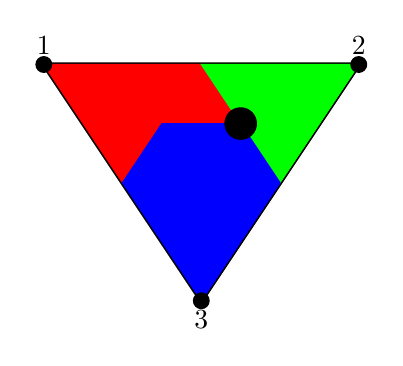
\begin{tikzpicture}
\draw[black, ultra thick] (2,3) -- (6,3) -- (4, 0) -- cycle;
\filldraw[color=red!100, fill=red!100] 
(2,3) -- (4,3) -- (4.5, 2.25) -- (3.5, 2.25) -- (3, 1.5) -- cycle;
\filldraw[color=green!100, fill=green!100] 
(4,3) -- (6,3) -- (5, 1.5) -- cycle;
\filldraw[color=blue!100, fill=blue!100] 
(3, 1.5) -- (3.5, 2.25) -- (4.5, 2.25) -- (5,1.5) -- (4, 0) -- cycle;
\filldraw[color=black!100, fill=black!100]
(4.5, 2.25) circle (0.2);

\filldraw[black] (2,3) circle (0.1) node[anchor=south]{1};
\filldraw[black] (6,3) circle (0.1) node[anchor=south]{2};
\filldraw[black] (4,0) circle (0.1) node[anchor=north]{3};

\end{tikzpicture}


У подібних розташуваннях очевидно завжди буде спільна точка, 
що і належить перетину. Тож, щоб перетин був порожній треба розставити 
множини послідовно (щоб були два кольори які не торкаються).


Очевидно подібне не можливо адже відрізки з'єднуючі вершини мають належати 
відповідним об'єднанням тож послідовно множини розставити не вийде.

\vspace{3 em}
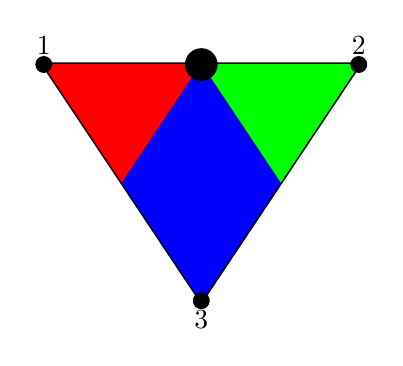
\begin{tikzpicture}
\draw[black, ultra thick] (2,3) -- (6,3) -- (4, 0) -- cycle;
\filldraw[color=red!100, fill=red!100] 
(2,3) -- (4,3) -- (3, 1.5) -- cycle;
\filldraw[color=green!100, fill=green!100] 
(4,3) -- (6,3) -- (5, 1.5) -- cycle;
\filldraw[color=blue!100, fill=blue!100] 
(3, 1.5) -- (4, 3) -- (5,1.5) -- (4, 0) -- cycle;
\filldraw[color=black!100, fill=black!100]
(4, 3) circle (0.2);

\filldraw[black] (2,3) circle (0.1) node[anchor=south]{1};
\filldraw[black] (6,3) circle (0.1) node[anchor=south]{2};
\filldraw[black] (4,0) circle (0.1) node[anchor=north]{3};

\end{tikzpicture}


З цього випливає, що в будь-якому разі перетин не буде порожній.
